\section{Graph-based naming}
\label{sec:graph}

%The MOTIF team (IRISA/Inria-Rennes and PUC Minas) considered a graph-based approach for naming the people which are both visible and heard (``speaking faces''). 
In this approach, all the \textit{speaking faces} of a video are the nodes of a complete and undirected graph $\mathcal{G}$, and each edge between two nodes is weighted by the similarity between their respective voices and/or the face tracks.
% The weight matrix $\mathbf{W}$ is therefore symmetrical. 
An initial tagging is done by associating to each face track the co-occurring name(s). Then propagation is performed according to the weights of the graphs using two different strategies, namely MOTIF-RW and MOTIF-MST (Fig.~\ref{fig:gbn}).

\begin{figure}[!htb]
 \centering
 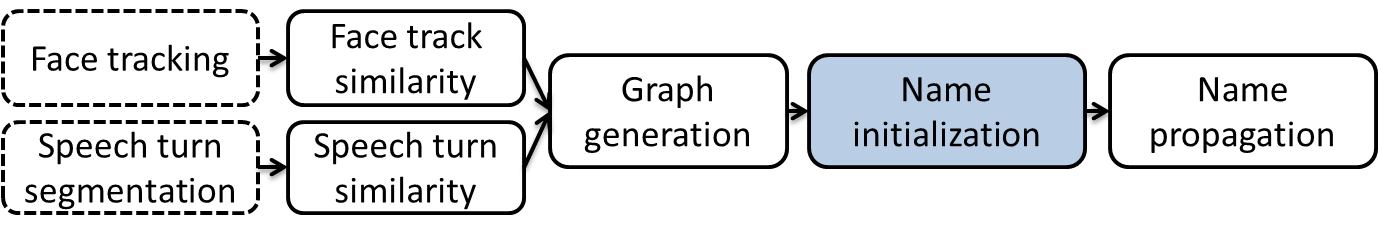
\includegraphics[width=1.\linewidth]{GBN.png}
\vspace*{-5mm}
 \caption{Graph-based naming process. Light blue boxes are when nodes in graph are initiated with names.}
\vspace*{-5mm}
 \label{fig:gbn}
\end{figure}

\subsection{Graph generation details}
\label{ssec:graph_gen}
A node is created for every \textit{speaking face} detected, namely when a face track temporally overlaps a speech segment by at least 60\%. If several speech segments overlap it, the face track is associated the one with the most overlapping one.
%
Edges between nodes are weighted using a measure of similarity deriving from the voice and/or face track similarities.

We compute the visual similarity $\sigma^V_{ij}$ as the cosine between the FaceNet embedding vectors $v_i$ and $v_j$ related to the face tracks of two nodes $N_i$ and $N_j$: $\sigma^V_{ij}=1/2+\frac{v_i\cdot v_j}{||v_i||*||v_j||}$, where $\cdot$ is the dot product and $||.||$ is the L2 norm.

The similarity $\sigma^A_{ij}$ between the speech segments of two nodes  $N_i$ and $N_j$ is computed as follows. Each speech segment is modelled with a 16-GMMs over MFCC features. An Euclidean-based approximation of the KL2 divergence, noted $\delta^A_{ij}$, is then computed between the two GMMs~\cite{Ben}, and turned into a similarity according to $\sigma^A_{ij}=\exp(\log{(\alpha)} \; \delta^A_{ij})$, where $\alpha = 0.25$.
%
The way two modalities can be combined is described in Sec. \ref{sec:multimodal}
%Section 6.2 describes how these similarities are combined into one, $\sigma^{AV}$, to fuse the .

\subsection{Name propagation}

Two different approaches are considered for the propagation of the initial tags: a random walk approach and a hierarchical one based on Kruskal's algorithm. In both cases, every node is associated a particular tag with a confidence score at the end of the propagation phase.

\subsubsection{Random walk (RW)}

This method implements a random walk algorithm with absorbing states, adapting~\cite{zhu2002}. Let $n$ be the number of nodes of $\mathcal{G}$, we compute the probability transition matrix $\mathbf{P}^0$ between all the nodes as $\mathbf{P}^0 = \mathbf{D}^{-1}\mathbf{W}$ where $\mathbf{D}$ is the diagonal {\it degree matrix} where $\mathbf{D}_{ii} = \sum_j \mathbf{W}_{ij}$, $1\leq i \leq n$. Nodes which are already tagged in $\mathbf{P}^0$ are set as \textit{absorbing states}, \textit{i.e.} if $i$ is a tagged node, $\mathbf{P}^0_{ii} = 1$ and $\mathbf{P}^0_{ij} = 0$. The random walk iteration is performed according to $\mathbf{P}^{t+1} = (1-\gamma) ~\mathbf{P}^0 ~ \mathbf{P}^{t} + \gamma ~\mathbf{P}^0$, where $\gamma$ is a parameter enforcing consistency with the initial state and slows down the walk (here $\gamma = 0.5$). When the random walk has converged, let $T$ be the final number of iterations. Each untagged node $u$ is then associated a tagged one $l^*$, where $l^*=\argmax_l{\mathbf{P}^{T}_{ul}}$. $\mathbf{P}^{T}_{ul^*}$ is considered as the confidence score related to the tagging of node $u$.

\subsubsection{Minimum spanning tree (MST)}
This method is based on the computation of a minimum spanning tree, using Kruskal's algorithm. The MST establishes a hierarchical partition of a set \cite{perret2015}. A new connected graph $\mathcal{G'}$ is derived from $\mathcal{G}$ with the same nodes but edge weights representing distances between them (functions of their respective similarities $\sigma^{AV}$). To propagate the initial tags, we start from a null graph $\mathcal{H}$ consisting in the nodes of $\mathcal{G'}$ only, and the following process is repeated, until all edges of $\mathcal{G'}$ are examined: from $\mathcal{G'},$ the unexamined edge $e$ corresponding to the smallest distance is chosen. If it does not link different trees in \color{black}$\mathcal{H}$\color{black},  skip it; otherwise, it links trees $T_1$ and $T_2$ (thus forming  $T_3$), and $e$ is added to the minimum spanning forest $\mathcal{H}$ being created. Three cases are possible: 
\textbf{I.}  None of $T_1, T_2$ is tagged: $T_3$ will not be tagged \textbf{II. } Only $T_1$ is tagged, with confidence score $C_{T_1}$: $T_1$'s tag is assigned to the entire  $T_3$ (\textit{i.e.,} to all its unlabelled nodes), with a confidence score $C_{T_3} = C_{T_1}\times(1-w_e), $ where $w_e$ is the weight of $e$ \color{black} in $\mathcal{G'}$. \color{black} \textbf{III. } Both $T_1$ and $T_2$ are tagged: one of the tags (of $T_1$ or of $T_2$) is picked (at random), and assigned to  $T_3$ with confidence scores as in case II. 


\endinput